\documentclass{report}
\usepackage{amsmath}
\usepackage{forest}
\usepackage{graphicx}
\title{Assignment One}
\author{Quin'darius Lyles-Woods}
\begin{document}
\maketitle
\section*{Problem One}

Compiling and running programs on the command line.

\begin{itemize}

	\item Open a command line window and compile the Java program with the ‘javac’ compiler.
	\item Verify that you have a compiled program using the ‘dir’ command (on Windows).
	\item Run the compiled program using the ‘java’ virtual machine.
	\item Compile and link the C++ program using the GNU C++ compiler.
	\item Verify that you have an executable file of the program.
	\item Execute the executable program.
	\item Show all your work.
\end{itemize}

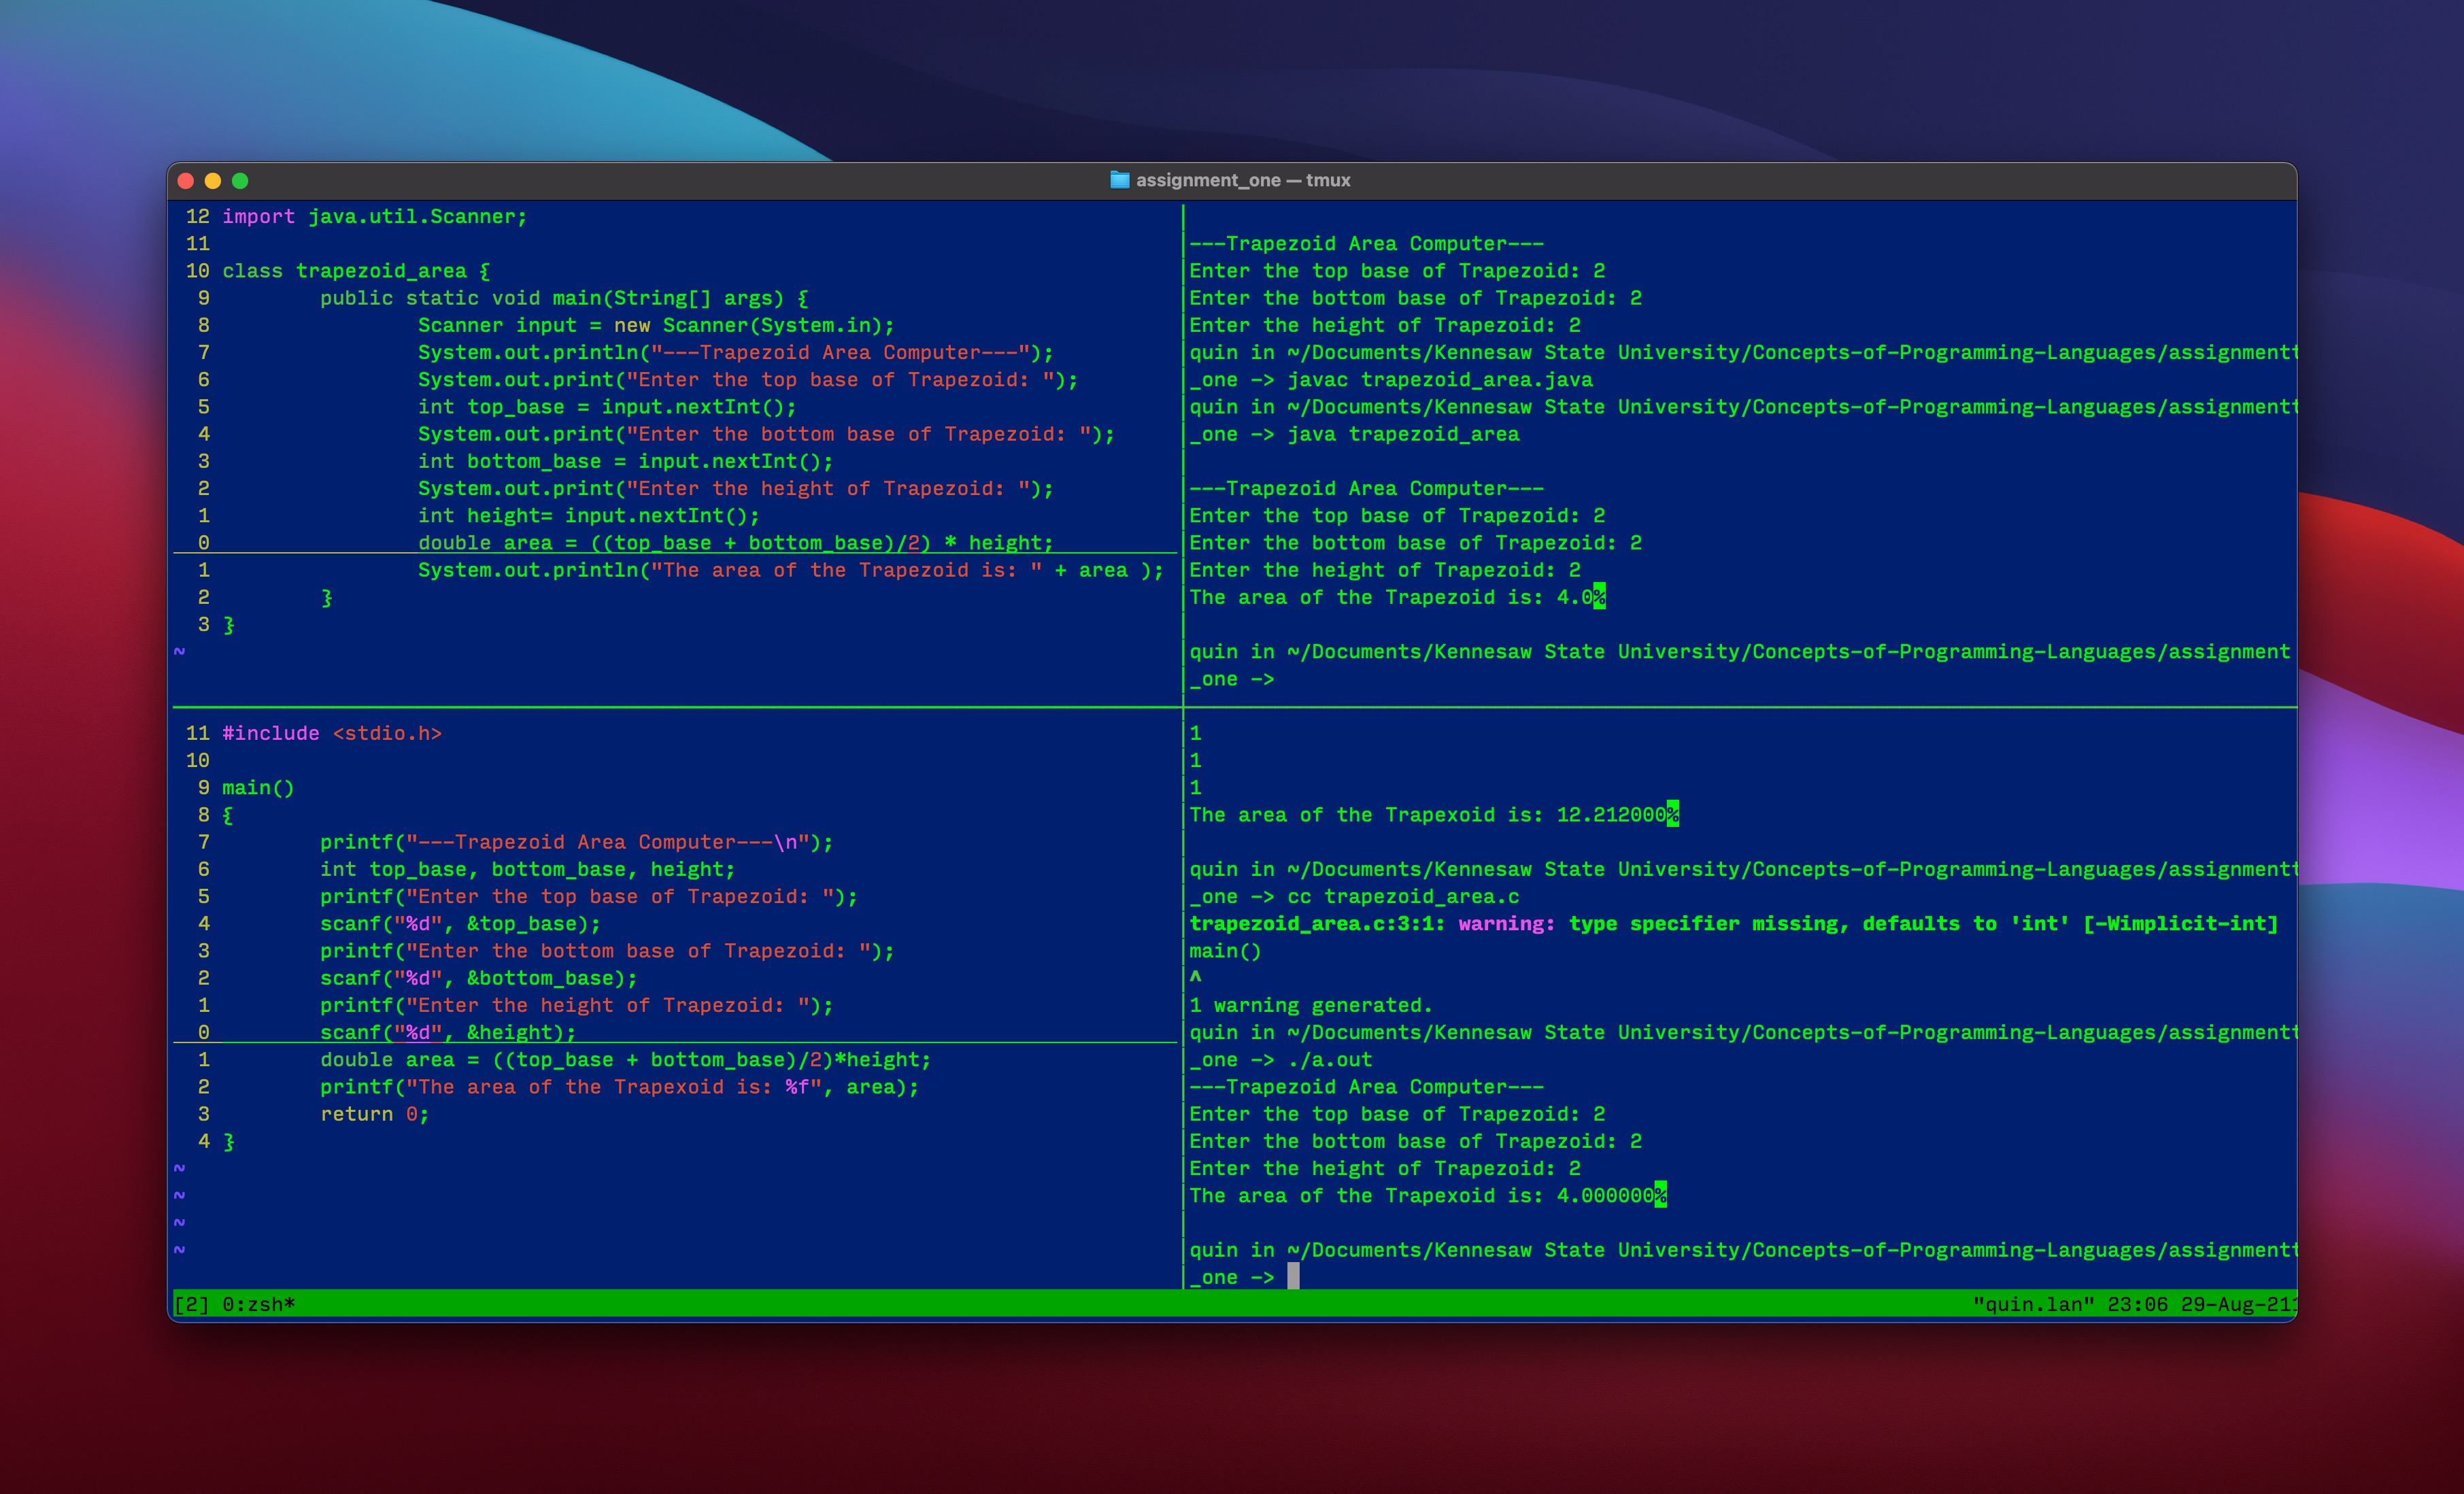
\includegraphics[width=\textwidth]{trapezoid_area}

\linebreak
\section*{Problem Two}
Rewrite the BNF of Example 3.4 to give + precedence over * and force + to be right associative.
\begin{align*}
<assignment> &\mapsto <id> = <expression>\\
<id> &\mapsto A\\
<id> &\mapsto B\\
<id> &\mapsto C\\
<expression> &\mapsto <expresion> * <term>\\
<expression> &\mapsto <term>\\
<term> &\mapsto <factor> + <term>\\
<term> &\mapsto <factor>\\
<factor> &\mapsto <expression>\\
<factor> &\mapsto <id>
\end{align*}
\section*{Problem Three}
Using the grammar in Example 3.4, show a parse tree and a leftmost derivation for each of the following statement: $A = B * (C * (A + B))$
\subsection*{Derivation}
\begin{align*}
<assignment> &\mapsto <id> = <expression>\\
&\mapsto A = <expression>\\
&\mapsto A = <id> * <expression>\\
&\mapsto A = B * <expression>\\
&\mapsto A = B * (<expression>)\\
&\mapsto A = B * (<id> * <expression>)\\
&\mapsto A = B * (C * <expression>)\\
&\mapsto A = B * (C * (<expression>))\\
&\mapsto A = B * (C * (<id> + <expression>))\\
&\mapsto A = B * (C * (A + <expression>))\\
&\mapsto A = B * (C * (A + <id>))\\
&\mapsto A = B * (C * (A + <B>))\\
\end{align*}
\subsection*{Parse Tree}
\begin{forest}
where n children=0{tier=word}{}
	[assignment
		[id
			[A]]
		[{=}]
		[expression
			[id
				[B]]
			[{*}]
			[expression
				[id
					[(C]]
				[{*}]
				[expression
					[id
						[(A]]
					[{+}]
					[expression
						[id
							[B))]]]]]]]
\end{forest}

\end{document}
